\chapter{重症患者的营养支持}

\section{前沿学术综述}

临床营养支持经历了40余年的发展,相关理论与应用技术得到了长足的进步。近年来,随着研究的深入和应用的推广,重症患者的临床营养支持,其目的已从单纯的“供给细胞代谢所需要的能量与营养底物,维持组织器官结构与功能”,拓展到调控应激状态下的高分解代谢,改善机体的免疫状态和保护器官功能等,即由“营养支持”向“营养治疗”发展。近年来,越来越多的研究注意到,疾病的严重状态或疾病阶段不同,具有不同的病理生理改变,对营养支持也有不同的需求。对于重症患者,熟悉机体疾病状态时代谢、免疫炎症反应以及器官功能的变化,适时采用合理、积极的营养支持治疗,已成为重症患者综合治疗策略中的一个重要的组成部分。

\subsubsection{重症患者的营养调理治疗}

临床实践表明,重症患者营养不良的发生迅速而普遍,并影响着其他并发症的发生与患者的病死率,成为预测重症患者预后不良风险的重要因素
\protect\hyperlink{text00028.htmlux5cux23ch1-27}{\textsuperscript{{[}1{]}}}
\textsuperscript{,}
\protect\hyperlink{text00028.htmlux5cux23ch2-27}{\textsuperscript{{[}2{]}}}
。因此,对重症患者实施及时、有效的营养干预,显得十分重要。迄今为止,营养支持并不能完全遏制和逆转重症患者严重应激时的分解代谢状态,对于单纯外源性补充蛋白质,重症患者的保存能力很差,而营养调理治疗有可能减少净蛋白的分解,促进蛋白质合成,改善潜在的和已发生的营养不良状态,防治相关并发症,已成为未来重症患者营养支持治疗的重要策略之一。

\subsubsection{早期肠内营养}

肠内营养(enteral
nutrition)可以维护肠道黏膜屏障、促进肠道蠕动与分泌,增加营养因子吸收进入肝脏合成蛋白质,减少细菌和毒素易位,降低肠源性感染和由此产生的“二次打击”,是符合生理的营养支持方式。重症患者肠内与肠外营养的荟萃研究显示,与肠外营养支持相比,肠内营养有助于降低重症患者感染性并发症的发生率,但对病死率的影响无差别。同时,与延迟肠内喂养相比,早期肠内喂养使重症患者肠内营养耐受性提高,热量摄入增加,感染并发症发生率也明显降低,并有降低患者病死率的趋势。尽管目前国际上对早期肠外营养(入院后3天内肠内营养达不到目标剂量即开始肠外营养)和延迟肠外营养(肠内营养7天达不到目标剂量再开始肠外营养)有争论,但最新的一项大宗多中心临床对照研究表明,当早期肠内营养难以满足病人能量需求时,延迟肠外营养补充较过早干预更能够加快病人恢复,减少并发症的发生
\protect\hyperlink{text00028.htmlux5cux23ch3-27}{\textsuperscript{{[}3{]}}}
。因此“想方设法开始早期肠内营养支持”已成为重症患者治疗的重要组成部分。

\subsubsection{严格血糖控制}

血糖升高是营养支持相关的代谢性并发症之一,重症患者发生率很高。严格血糖控制是重症患者营养支持策略的重要组成部分。强化胰岛素治疗严格控制血糖是近年来重症医学领域的一个关注重点。临床研究表明,控制重症患者的血糖水平,可明显降低感染与器官功能障碍(如急性肾衰竭等)的发生率,缩短机械通气时间与住院时间、降低病死率。目前认为,无论采用何种形式的营养支持,均应配合强化胰岛素治疗策略,以提高营养支持治疗的安全性、有效性。推荐血糖浓度维持在8.0mmol/L左右,并积极预防低血糖的发生。

\subsubsection{发挥营养素的药理学作用(免疫营养)}

严重应激后,患者的部分营养素发生明显改变,并可能影响患者的预后。这类营养素被认为是疾病的治疗药物,而不再是单纯的营养补充,其中一些营养素可以特定方式刺激免疫细胞,增强免疫应答能力,维持正常或适度的免疫反应,调控细胞因子的产生和释放,从而减轻有害的或过度的炎症反应,维持肠道屏障功能,这类营养素被称为免疫营养素。在标准营养配方的基础上添加某些特殊免疫营养物质,利用其药理学作用而达到治疗和调节机体代谢和免疫功能的目的,即免疫营养学。

目前,研究较多并用于临床的特殊营养素有谷氨酰胺(glutamine)、精氨酸、ω-3脂肪酸(鱼油)、核苷与核苷酸、膳食纤维,以及含有乳酸杆菌、双歧杆菌的生态免疫营养素等。近年来,免疫营养制剂越来越多地应用于肠内与肠外营养支持,获得了较理想的结果,但有许多问题尚需进一步探讨。

综上所述,重症患者的营养支持近年来的发展突出体现在以下几个方面:①限制应激反应期能量的供给量;②及早开始营养支持;③优先选择肠内营养,以在更好实现营养补充的同时,维持肠道、免疫、内分泌等生理功能;④提倡联合营养的概念,即在肠内供给不足或不耐受肠内营养时,可给予肠外营养;⑤强化胰岛素治疗是实现重症患者安全有效的营养支持的必要策略;⑥除营养底物的补充外,还应重视营养素的药理作用。

\section{临床问题}

\subsubsection{重症患者应激后的生理与代谢反应有何特点?}

机体遭受创伤、烧伤、感染以及大手术打击后,会发生一系列病理生理反应和代谢改变,可表现为体温升高、呼吸频率及心率增快、心排出量增加、氧输送与氧耗增加、血管通透性增加、外周血白细胞增多等,同时机体代谢状态发生迅速变化,呈现高代谢特征,即能量消耗迅速增加、糖异生增加、血糖升高、脂肪动员加速、蛋白质迅速分解,导致净氮丢失增加及负氮平衡。实际上,应激情况下机体代谢改变也是全身炎症反应的一部分。代谢紊乱的程度、持续的时间与应激和炎症反应的程度密切相关。

目前认为,参与和调节应激反应的炎症介质主要包括激素、细胞因子和脂质介质三类(表\ref{tab22-1}),这些因素通过放大和负反馈机制相互作用。细胞因子和脂质介质可能是激素变化的启动介质或炎症免疫反应的中心。垂体-肾上腺轴的过度兴奋导致儿茶酚胺、胰高血糖素、肾上腺皮质激素等分解激素分泌增加,生长激素与胰岛素的分泌增加或不变,但胰岛素样生长因子(IGF-1)合成减少,使机体促合成激素相对减少。巨噬细胞、淋巴细胞激活释放肿瘤坏死因子(TNF)α、白细胞介素(IL)-1、IL-6、干扰素(IFN)等细胞因子,影响糖、蛋白质、脂肪等营养物质的代谢。脂质介质如前列腺素E\textsubscript{2}
(PGE\textsubscript{2} )、血栓素A\textsubscript{2}
(TXA\textsubscript{2}
)、白三烯B4及血小板活化因子的产生增加,参与调节体内营养物如蛋白质的合成等。

\begin{table}[htbp]
{\centering
\caption{参与和调节应激反应的激素和介质}
\label{tab22-1}
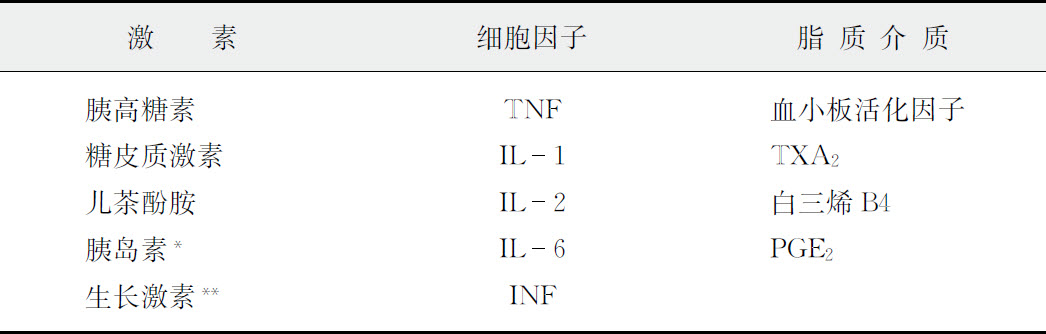
\includegraphics{./images/Image00256.jpg}}

\footnotesize
* 分泌减少或胰岛素抵抗。

** IGF-1合成不足。
\end{table}



\subsubsection{重症患者应激导致哪些能量代谢改变?}

影响重症患者能量消耗和呼吸商(底物氧化率)的相关因素较多,除与病种和病情严重度、年龄、身高、体重相关外,还与患者的体温、镇静或(和)肌松药物的应用以及机械通气支持等显著相关。即使同一疾病在不同阶段,机体的能量消耗亦有不同。择期手术患者静息能量消耗(resting
energy
expenditure)增加0~10%;外科严重创伤、感染患者静息能量消耗增高30%左右;创伤、感染患者静息能量消耗增高20%~50%。全身性感染的不同时期,能量消耗的变化也不相同(表\ref{tab22-2})。烧伤患者尤其是大面积烧伤者,能量消耗的增加较为明显,与烧伤面积相关。烧伤面积>40%时,静息能量消耗可增加100%,甚至更高。即使烧伤面积、深度相似,不同个体之间能量消耗的变化也可达30%~40%。所以,不论何种用于临床患者的能量消耗/需要判断公式,都可能与实际需要存在一定偏差,需要个体化评估和调整。有条件时,可通过代谢车(间接能量测定法,indirect
calorimetry)测定实际静息能量消耗。

\begin{table}[htbp]
\centering
\caption{感染程度与能量代谢率(%)的关系}
\label{tab22-2}
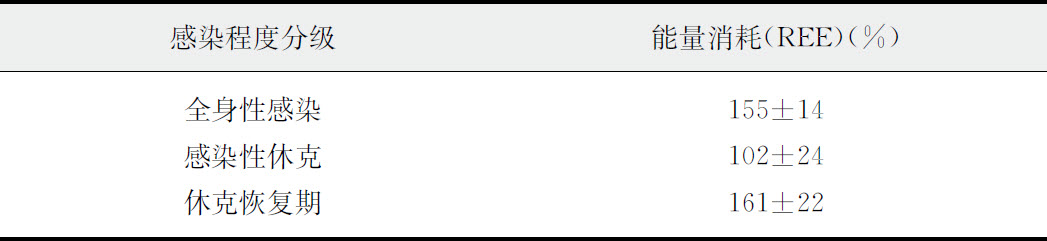
\includegraphics{./images/Image00257.jpg}
\end{table}

代谢车亦称为代谢监测系统,它通过测定机体在单位时间内消耗的氧气和产生的二氧化碳,计算得出静息能量消耗和呼吸商,并了解三大类营养物质在一定时间内氧化代谢的量和相对比例。

每次使用代谢车测定机体静息能量消耗前,都要对仪器分别进行容量、氧气分析仪和二氧化碳分析仪定标。头罩法是目前国际上最常用的测量方法,采用该法测量时患者痛苦小,耐受性好,生理无效腔小,对呼吸的干扰较少,特别适用于昏迷和意识不清等不能主动配合检测的患者。对于机械辅助通气的重症患者,可使用特殊的连接装置将呼吸机和代谢车连接起来,呼吸机测定患者吸入的氧气量和气体容量,呼出气则由代谢车进行自动分析。

总能量消耗(total energy
expenditure)指在静息能量消耗基础上,加上食物特殊动力作用和活动时的能量消耗。重症患者往往不能经肠道喂养或经口进食,不能处于真正的静息状态,其静息能量消耗相当于代谢能量消耗(metabolic
energy
expenditure),与总能量消耗比较接近。代谢车测定的结果显示,重症患者的实际能量需要(即总能量消耗)仅较静息能量消耗增高10%左右,总能量消耗=静息能量消耗×1.03±0.071。

由于重症患者的实际能量消耗和呼吸商与普通患者、健康人均有较大差异,使用代谢车进行评估与监测,可以帮助解决重症患者营养支持用多少量、用什么配方的问题,减少重症患者营养配方不合理带来的并发症的问题。

\subsubsection{重症患者应激状态下碳水化合物的代谢有何变化?}

体内主要的碳水化合物是葡萄糖。应激时能量消耗的增加使葡萄糖的需要量增加,而体内糖元储存有限,为200~400g,24~36小时内即可耗尽。之后,机体将通过动员储存的脂肪产生三酰甘油,同时肌肉与内脏蛋白质分解,释放大量氨基酸,在肝脏内经糖异生途径产生葡萄糖,使血糖升高,引起“应激糖尿病”。

不同应激状态,葡萄糖的产生和利用亦有不同。创伤后的重症患者,葡萄糖的产生和利用均是增加的。乳酸、丙氨酸是合成葡萄糖的前体,葡萄糖消耗增加,乳酸产生亦增多,后者被肝脏吸收转化为葡萄糖。同时,应激时的肌肉蛋白质大量分解与脂肪动员增加,脂肪组织产生的丙氨酸是肌肉产生量的1/3,肝脏吸收丙氨酸并使之转化为葡萄糖。所以,创伤后肝葡萄糖的生成率增加,体内糖生成量达每分钟2~5mg/kg,较正常增加150%~200%。虽然胰岛素分泌正常甚至增高,但机体对葡萄糖处理能力受到抑制,导致创伤后高血糖和胰岛素耐受现象。

全身感染患者葡萄糖异生增加等因素,使血糖升高,血葡萄糖增高大于胰岛素增高,但葡萄糖的氧化代谢发生障碍,葡萄糖利用受限。新近的研究提示,感染患者糖代谢改变与细胞因子介导的外周组织葡萄糖的摄取、转运障碍有关,其机制为细胞表面胰岛素受体或葡萄糖载体的作用受抑制。

可见,应激时的高血糖是糖代谢紊乱的特点。若过量摄入葡萄糖,势必加重糖代谢紊乱及器官(肝、肺等)功能负担,如二氧化碳产生增加,呼吸商升高,呼吸负担加重,糖元储存增加。当超过能量消耗和糖元储存所需要的糖量时,葡萄糖将转化为脂肪酸,进一步影响脂肪代谢,使脂肪氧化转向脂肪合成,并可导致肝脏脂肪堆积及淤胆。

\subsubsection{重症患者应激状态下蛋白质与氨基酸的代谢有哪些特点?}

蛋白质分解代谢高于合成代谢及负氮平衡是创伤、烧伤与全身感染患者蛋白质代谢特点。应激时,细胞因子与神经内分泌的作用,常常导致广泛的蛋白质分解和快速、严重的氮耗竭,Cerra将这种机体通过分解自体组织获取能量的现象称为“自身相食(autocannibalism)”。蛋白质分解增加,特别是骨骼肌、肠道等体细胞团的丢失,进一步影响机体器官组织结构与功能,导致骨骼肌萎缩、呼吸驱动力下降、肠黏膜萎缩及屏障功能受损、免疫机能降低及血浆蛋白降低。人体内蛋白质含量约为11kg,具有维持肌肉功能(呼吸肌和心肌等)的重要作用。严重应激时,尿氮排出量可达35~40g/天,相当于1kg瘦体组织。大量的瘦体组织和骨骼肌、肠道等体细胞团的消耗使重症患者病死率明显增加。分解激素水平升高,促使体内的蛋白质分解。细胞因子除促进蛋白质分解外,还影响蛋白质合成,使肝脏合成清蛋白、转铁蛋白、前白蛋白受抑制。感染、创伤时肿瘤坏死因子和白介素(IL)-1等通过抑制mRNA转录,使清蛋白合成减少。而急性相蛋白(如C反应蛋白,α胰蛋白酶等)合成增加,将进一步增加氮的需要量。

感染、创伤后的血浆氨基酸浓度变化与体内代谢反应及病程相关。受损组织蛋白质分解,导致血浆氨基酸浓度升高。感染未控制期间,血浆氨基酸水平升高,反映体内分解代谢增强,感染控制后逐渐恢复正常。肝脏功能受抑制时,芳香族氨基酸和含硫氨基酸(蛋氨酸、半胱氨酸)的血浆浓度升高。应激时血浆及细胞内氨基酸变化较突出的是谷氨酰胺和支链氨基酸。细胞内与血浆中氨基酸含量受不同疾病与代谢状态影响,而细胞内氨基酸浓度变化与血浆氨基酸浓度改变可能并不一致。严重分解代谢状态下,骨骼肌内蛋白质大量分解,支链氨基酸、芳香族氨基酸和蛋氨酸均明显增加,但血浆内支链氨基酸的变化则相反,多数重症患者肝内支链氨基酸的浓度亦是降低的。支链氨基酸的这一变化,与严重应激状态下肝脏功能受抑制,使其对一些代谢物质的处理能力降低有关。特别是肝功能受损时不能代谢由肌肉组织释放的大量芳香族氨基酸,导致血浆中芳香族氨基酸和蛋氨酸的浓度增加,后者竞争性地抑制肌肉支链氨基酸的流出;同时,由于支链氨基酸能在肝外代谢产能,致使血浆内支链氨基酸浓度更为降低。

\subsubsection{重症患者应激状态下脂肪代谢有哪些变化?}

创伤与感染等应激时,儿茶酚胺水平升高促使体内脂肪动员与氧化加速,可达正常速度的200%。脂肪分解产物三酰甘油、游离脂肪酸和甘油成为主要的供能物质。胰岛素水平的降低亦刺激游离脂肪酸释放。结果使血浆三酰甘油、游离脂肪酸浓度增加。

细胞因子亦参与了脂肪代谢的调节。肿瘤坏死因子和白细胞介素-1通过抑制脂蛋白酯酶的活性,使三酰甘油浓度升高。肿瘤坏死因子α还可直接作用促使儿茶酚胺分泌增加,而白介素-1还可促进胰岛素的分泌。

血浆三酰甘油和游离脂肪酸水平升高,三酰甘油的更新率增加,并参与能量的产生。游离脂肪酸在肝内再循环,使极低密度脂蛋白三酰甘油的产生增加,外周脂肪细胞的摄取减少。严重感染的患者,细胞因子促进肝脏对脂肪酸的重新合成,同时摄取血浆中游离脂肪酸增加。可导致肝细胞内过多的三酰甘油聚积,形成脂肪肝。

此外,应激后肉毒碱合成减少,停止摄食又使其摄入降低,加上排泄增加,导致体内肉毒碱水平下降,严重感染患者更为突出,从而使长链三酰甘油(LCT)的氧化利用受到影响。此时若不恰当地供给外源性脂肪(尤其是LCT),可导致脂肪超负荷。

\subsubsection{重症患者应激状态下体内微量营养素的代谢有何变化?}

重症患者体内微量元素异常释放与重新分布,加之摄入减少与排泄异常,使微量元素的血浆发生浓度变化。细胞因子参与了感染、创伤以及多器官功能障碍综合征时微量元素的代谢调节。白细胞介素-1可引起微量元素结合蛋白由细胞内向细胞外释放,导致微量元素向血管外间隙转移,使血清铁(Fe)、锌(Zn)、硒(Se)含量降低,而血铜(Cu)含量常常升高。微量元素变化可影响碳水化合物、脂肪、蛋白质代谢、肠道形态学及免疫功能。

(1)铁 感染时血清铁含量降低,肝脏铁含量升高。乳铁蛋白是一种铁结合蛋白,正常情况下主要存在于中性粒细胞质粒中。乳铁蛋白从转铁蛋白上鳌合铁形成复合物,后者进入肝脏被肝细胞识别并加快清除,使血清铁含量下降。铁缺乏可影响机体免疫功能,如引起T淋巴细胞数量与功能下降、中性粒细胞杀菌力降低,并可导致贫血。

(2)锌 感染、烧伤等患者易发生低锌血症。内毒素与细胞因子促使肝脏及其他组织合成急性相蛋白和金属硫蛋白(金属甲硫氨酸),血锌利用增多,锌由血向肝脏转移,导致血锌减少。此外,约60%的锌与清蛋白疏松结合,感染等应激时清蛋白的大量分解及合成受抑制,尿、汗的丢失增加均可加重血锌的降低。

肝脏是锌缺乏最敏感的器官之一。低锌影响碳水化合物、脂肪及蛋白质代谢酶的活性,进而影响营养代谢。锌的缺乏还可导致肠道形态学改变,包括绒毛高度、腺窝深度降低,固有层细胞浸润和肠黏膜损害。此外,锌是对免疫功能影响突出的微量因素之一。缺锌使T淋巴细胞,尤其是T辅助细胞数量与功能下降。缺锌还可使巨噬细胞吞噬与杀菌能力下降、中性粒细胞游走功能降低。

(3)硒 硒是谷胱甘肽过氧化酶的组成部分,主要起防止过氧化损伤的作用。全身性感染等重症患者血硒水平呈不同程度的下降,与硒由血浆再分布到组织有关。血浆硒明显下降,可降低谷胱甘肽过氧化酶活性,使机体抗氧化能力受损。此外,硒还参与辅酶A、泛醌及其他许多代谢酶的组成,影响其生物活性,如能量代谢(ATP)及维生素A、维生素D、维生素E、维生素K的吸收与消耗。硒还具有促进生长、维护心血管功能,以及参与机体免疫功能的作用。硒缺乏可使巨噬细胞、中性粒细胞杀菌能力下降,B细胞产生抗体减少。

(4)铜 严重感染、烧伤患者血清铜水平多升高。铜吸收后与清蛋白疏松结合,在肝脏合成铜蓝蛋白,释放入血并转运到各器官组织,以提供铜。铜蓝蛋白是运输铜和维持组织中铜水平的主要蛋白,血浆中50%的铜与铜蓝蛋白结合。感染时铜蓝蛋白合成增加,血铜增加。反复感染者铜蓝蛋白缺乏,亦可使血铜变化不明显。铜参与体内一些酶的组成,包括超氧化物歧化酶、细胞色素氧化酶、磷脂化酶、琥珀酸脱氢酶、赖氨酸氧化酶、多巴胺β羟化酶等,血铜改变将影响酶的活性。

(5)维生素 严重创伤、感染、出血及低灌注等可导致组织器官缺血/再灌注损伤,使血浆中谷胱甘肽(GSH)及维生素E、维生素C、维生素A等抗氧化剂消耗增多,浓度明显降低,导致机体抗氧化能力严重受损,并使抗氧化剂需要量明显增加。维生素C需要量可达推荐量的10倍。近年来,在重症患者营养支持中,抗氧化维生素的补充已逐渐得到重视。

\subsubsection{如何掌握重症患者营养支持的指征?}

在遭受严重创伤、感染打击后出现的一系列免疫炎症和内分泌反应,使人体原有内稳态的平衡破坏,机体的代谢状态乃至机体的组成亦迅速发生变化,营养状况迅速下降及发生营养不良是重症患者普遍存在的现象,并成为影响重症患者预后的独立因素。临床研究表明,及时、合理的营养支持有助于降低重症患者营养不良的发生及改善预后;相反,延迟的营养支持将导致累积能量负平衡的加重及长时间的营养不良,并难以为后期的营养支持所纠正。营养摄入不足和蛋白质能量负平衡与发生营养不良及血源性感染相关,并延长住重症医学科及住院时间,增加医疗费用
\protect\hyperlink{text00028.htmlux5cux23ch1-27}{\textsuperscript{{[}1{]}}}
。因此,营养支持已成为危重症患者生命支持治疗中的一个重要方面。

大多数重症患者都有接受营养支持治疗的指征,但缺乏量化的评价系统,学者们试图寻找重症患者营养评价的工具去具体判断营养风险,为重症患者的营养治疗提供依据。“Can
we
feed”重症病人营养评估量表可以帮助我们很好地评估病人的营养状况及营养支持实施的效果,必将成为重症病人营养状况评估的常用工具
\protect\hyperlink{text00028.htmlux5cux23ch2-27}{\textsuperscript{{[}2{]}}}
。控制应激状态、全身性感染与炎症反应程度对于有效的营养治疗是至关重要的,否则单靠营养治疗并不能改善患者的预后。为了维持细胞的代谢与器官的功能,重症患者原则上应在经过初期的治疗,血流动力学稳定,水、电解质与酸碱失衡得到初步纠正后,及早给予营养支持,即在复苏与初期治疗后24~48小时即可开始。应用营养支持前需对患者的代谢状态、脏器功能进行评估,了解这次疾病前有关影响营养状态的病史,如有无肝病、心力衰竭、肾衰竭、肿瘤以及糖尿病、高脂血症等。

存在以下情况时均不宜开始营养支持:①在复苏早期,特别是容量复苏尚不充分,血流动力学尚未趋于稳定时;②存在严重的代谢紊乱(应激性高血糖尚未得到有效的控制、存在严重酸中毒等);③存在严重肝功能障碍、肝性脑病、严重氮质血症等时,营养支持很难有效实施。

\subsubsection{如何选择重症患者营养支持的方式?}

肠外营养与肠内营养是临床营养支持的两种方式。重症患者营养支持方式选择的原则是:当肠道有功能且能安全使用时,应该使用肠道。肠内营养提供机体所需营养量的15%~20%,就能够起到维持肠黏膜屏障、调节免疫功能的作用。即优先使用肠内营养。

(1)肠外营养 这是一种非生理的治疗途径。过去30年中肠外营养得到了长足的完善与发展,使许多合并肠功能障碍患者的营养状况乃至生命得到维持,人们对肠外营养在肠功能维护、肝脏与免疫功能等方面的不利影响与缺陷也有了更充分的了解,肠外营养费用高于肠内营养。原则上,对于存在胃肠道解剖异常与功能障碍的重症患者,肠外营养支持仍然是综合治疗的重要组成部分。研究显示,合并有营养不良而又不能通过胃肠道途径提供营养支持的重症患者,如不给予及时、有效的肠外营养支持,死亡危险将增加3倍。

(2)肠内营养 肠内营养是为机体提供营养物的符合生理的营养支持方式,尤其在支持、维护肠道屏障功能,增加肠道与门脉血流,促进肠道运动、分泌、消化功能与释放胃肠激素等方面,其作用优于肠外营养。临床研究表明,接受肠内营养的重症患者,其发生感染性并发症的风险比接受肠外营养者为低。此外,肠内营养还具有价格低廉、实施相对简单、相关并发症少等优点。

有关重症患者肠外与肠内营养应用比较的荟萃分析研究和临床经验显示
\protect\hyperlink{text00028.htmlux5cux23ch2-27}{\textsuperscript{{[}2{]}}}
,肠外营养与感染性并发症的增加有关,而接受肠内营养的重症患者感染风险比接受肠外营养者为低。临床研究显示,早期应用肠内营养,感染性并发症的发生率较低,住院时间缩短。但并非所有重症患者均能获得同样效果,特别是在比较肠内营养与肠外营养对改善预后、降低住院时间与机械通气时间等方面,尚缺乏有力的证据。这可能与重症患者病情复杂、影响因素多有关,如所患疾病的情况、营养供给量及营养支持相关并发症等。有关外科重症患者营养支持方式的循证医学研究表明,80%的患者可以耐受完全肠内营养(total
enteral
nutrition),另外10%可接受肠外营养和肠内营养混合形式营养支持,剩余的10%不宜使用肠内营养,是选择全胃肠道外营养的绝对适应证。应该指出,重症患者肠内营养不耐受的发生率高于普通患者,回顾性调查显示,仅有50%左右接受肠内营养的重症患者可达到目标喂养量,每天104.6kJ/kg
\protect\hyperlink{text00028.htmlux5cux23ch4-27}{\textsuperscript{{[}4{]}}}
(1 kcal=4.18kJ)。

对于营养支持方式的选择,主要依赖于具体的病情和疾病状态,特别是肠功能状态。在肠功能障碍,特别是在严重创伤的早期或是腹部创伤、腹腔存在较严重感染时,肠外营养便成为主要的营养供给途径,为机体提供必需的营养物质。可见,肠外与肠内两大途径起着互补作用,需合理选择。对胃肠道消化吸收及运动功能降低或血容量不稳定、内脏血流减少的患者,应限制肠道喂养量,以防滞留或误吸。当胃肠道功能障碍,不能进行或不能达到充足的肠道喂养时,应及早进行完全或部分肠外营养,以保证患者能获得足够的液体、能量与各种营养物质的补充。一旦胃肠功能恢复,应及早由肠外营养过渡到肠内营养。

经管饲提供肠内营养是重症患者最理想的营养支持途径。在血流动力学稳定及胃肠道有功能的前提下,应及早开始肠道喂养。一般认为,入重症医学科或患病后24~48小时开始的肠道喂养称为早期肠内营养。应激后的代谢改变使重症患者能量消耗与营养丢失明显增加,如不及早处理,会很快出现能量负平衡(负债),并进行性加重,后期也难以通过补充纠正,将延长重症医学科住院时间,增加医疗费用。

然而重症患者胃肠排空障碍和肠内营养不耐受的发生率较高,常常影响早期肠内营养的实施。常见因素包括肠内营养前及肠内营养实施过程中胃残余量过多,镇静、儿茶酚胺药物的应用等。在这类患者中,若过分强调肠内营养,反而会使肺炎发生率增加、住院时间延长。

可见,早期肠内营养是重症患者理想的营养支持方式,对于肠内营养不耐受的重症患者,亦应及时给予肠外营养,以免加重营养不良。为保证肠内营养使用的安全有效,计划性的实施方案对于肠道喂养的合理应用是必要的,包括对重症患者肠道能否使用的评估、营养通路与营养制剂的选择、使用方法、肠内营养耐受性与相关并发症的判断以及营养液输注的管理等。

\subsubsection{重症患者的能量供给应选择高热量还是低热量营养支持?}

严重应激后,包括细胞因子在内的大量炎症介质释放,促分解代谢激素分泌增加,导致分解代谢明显大于合成代谢,机体的能量消耗增加,出现持续的负氮平衡、脂肪动员以及应激性高糖血症。鉴于应激期(尤应激早期)的代谢改变特点,早年营养与能量供给的原则是增加能量的供给与“满足”能量代谢的“需求”,临床上常根据体重给予较高的能量以达到此时的能量消耗量,一般在每天167.3~209.2kJ/kg,或根据Harris-Benedict公式:

\[
  \begin{array}{l}
\text{男性基础能量消耗(kcal/24h)}=66.5+13.8\times W+5\times H-6.8\times A  \\
\text{女性基础能量消耗(kcal/24h)}=65.5+9.6\times W+5\times H-4.7\times A  
  \end{array}
\]

式中,W是以kg为单位的体重,H是以cm为单位的身高,A是患者年龄(岁),计算出基础能量消耗后再乘以一定的应激系数(1.5~2.0)。不管上述何种方法,都被后来的实际能量代谢测定研究证实,其能量的补充往往超过机体的代谢能力,甚至会加重应激后的代谢紊乱与脏器功能损害,并且与重症患者并发症发生率及病死率相关。近年来,能量代谢研究特别是应用间接能量测定法(metabolic
cart,代谢车)及其他形式的氧耗状态测定实际能量消耗发现,应激患者代谢率的增加常比以往估计的要低。此外,除了要考虑应激后的能量消耗量外,机体对补充的能量与营养底物的利用能力又是另一需要考虑的问题,而一些相关研究显示,适当限制应激后的能量供给,营养支持的效果与安全性得到改善。

目前,国际上多数学者认为,合并全身炎症反应的急性重症患者,能量供给在每天83.7~104.6kJ/kg,是大多数重症患者应激早期能够接受并可实现的能量供给目标,即所谓“允许性”低热量。目的在于避免营养支持相关并发症,如高血糖、高碳酸血症、胆汁淤积与脏器功能损害等。随着应激与代谢状态稳定,能量供给应适当增加,BMI<30,达每天104.6~125.5kJ/kg;BMI>30,可达46.0~58.6kJ/kg。重症患者由于常合并水肿及活动限制,其体重计算使用实际体重
\protect\hyperlink{text00028.htmlux5cux23ch2-27}{\textsuperscript{{[}2{]}}}
。

\subsubsection{肠外营养液的成分包括哪些?如何补充?}

营养支持的成分除水外,可分为大营养素(macronutrient)与微营养素(micronutrient)两大类。

(1)大营养素(或常量营养素) 主要指碳水化合物、脂肪、蛋白质(或氮)。碳水化合物是非蛋白质热量(non-protein
calorie)的主要来源之一,体内主要的碳水化合物是葡萄糖,应激后的糖代谢改变是糖的利用下降和产生增加,不论是否合并有糖尿病,许多重症患者出现血糖明显升高,并影响预后。大量补充葡萄糖会加重糖代谢紊乱及脏器功能损害的危险。过多热量与葡萄糖的补充还会增加二氧化碳的产生、增加呼吸肌做功、肝功能损害与淤胆发生等,特别是对合并有呼吸系统损害的重症患者。总之,葡萄糖的供给应参考机体糖代谢状态与肝、肺等脏器功能。应降低非蛋白质热量中的葡萄糖补充,葡萄糖的补充量一般占非蛋白质热量的50%~60%;葡萄糖∶脂肪比例保持在60∶40~50∶50,此外,要强调联合强化胰岛素治疗、严格控制血糖水平。

脂肪通常是非蛋白热量的另一主要来源,基于对严重应激后代谢紊乱的认识,重症患者营养支持的一个原则是降低非蛋白质热量中的葡萄糖热量,以糖脂双能源满足能量的供给,目的在于减轻葡萄糖的代谢负荷,保护脏器功能,提供必需脂肪酸。危重症患者脂肪供给量一般为每天1~1.5g/kg,但应参考机体对糖与脂肪的代谢能力,监测脂肪廓清与血糖水平以及肝肾功能。对合并脂代谢障碍者(如重症胰腺炎)及老年患者,应降低脂肪乳剂的补充量。

代谢过程中,不同的脂肪酸对肉毒碱的依赖程度不同。在脂肪酸β氧化中,脂酰辅酶A进入线粒体氧化需肉毒碱转运,而在感染等应激状态及肝功能障碍时,肉毒碱产生较少,或尿中排泄增加,可导致血浆与组织中肉毒碱水平下降,这在严重感染患者更为突出,从而使长链甘油三酯氧化受到限制,因而不恰当地供给外源性脂肪(尤其是长链脂肪乳),可导致脂肪超负荷及廓清障碍。中链甘油三酯进入线粒体代谢时对肉毒碱依赖性小,易被上皮细胞结合的蛋白酯酶和肝内酯酶水解,具有氧化迅速,且不在肝脏及外周组织中浸润及形成脂肪组织等优点。此外,中链脂肪酸与白蛋白结合疏松,有较高的可溶性,使其容易被组织摄取;并且,中链脂肪酸同白蛋白上胆红素结合位点的亲和力较长链脂肪酸低,对胆红素代谢干扰小,可作为高胆红素血症患者的供能物质。

目前临床常选择的商品化静脉脂肪乳剂种类很多,但根据碳链长短,可分为含长链甘油三酯(18~24碳)的脂肪乳剂、中长链混合脂肪乳剂和含中链甘油三酯(6~12碳)的脂肪乳剂。长链脂肪乳中含有必需脂肪酸(essential
fatty
acid,EFA)。由于中链甘油三酯不依赖肉毒碱转运进入线粒体,有较高氧化利用率,更有助于改善应激与感染状态下的蛋白质合成。因而,在严重创伤、感染的重症患者及肝功能障碍、黄疸患者的营养支持中,较传统的长链甘油三酯脂肪乳剂更具有优势。

氨基酸溶液作为肠外营养液中的氮源,是蛋白质合成的底物来源,平衡型氨基酸是临床常选择的剂型,它不但含有各种必需氨基酸,也含有各种非必需氨基酸,且各种氨基酸的比例适当,具有较好的蛋白质合成效应。支链氨基酸是肝外代谢的氨基酸,因此应用支链氨基酸强化的复方氨基酸液有助于减轻肝功能障碍患者的肝脏代谢负担,并有助于调整血浆氨基酸谱和防治肝性脑病。曾有人认为它亦有助于改善创伤患者的蛋白质合成,但临床研究并未证实应用强化支链氨基酸(含36%~40%支链氨基酸)的复方氨基酸液的全肠外营养支持,在节氮和促进蛋白质合成方面有特殊优势。重症患者肠外营养时,蛋白质补充量及热氮比构成的原则为:蛋白质供给量体重指数<30时为每天1.2~2.0g/kg,相当于氮每天0.32g/kg,体重为目前的实际体重;热氮比418.0~627.6kJ∶1gN。30<体重指数<40时为每天2.0g/kg,体重指数>40时为>每天2.5g/kg,此时参照的体重为理想体重。

营养方案要结合重症患者的特点,营养液的容量应根据病情及每个患者具体需要,参照液体平衡与前负荷状态综合考虑确定,并根据需要给予及时监测和调整。

每日常规所需要的电解质主要包括钾、钠、氯、钙、镁、磷。接受全肠外营养的重症患者,每日补充生理剂量的电解质,但当疾病导致额外丢失增加时,应注意监测、补充。

(2)微营养素 维生素、微量元素等体内含量低、需要量少,故被称为微量营养素,但它们同样有着重要的生理作用。

维生素 维生素C参与蛋白和组织细胞间质的合成,有利于减轻组织损伤及促进其修复。维生素B\textsubscript{1}
的需要量与摄入的能量成比例地增加;维生素B\textsubscript{2}
的排出量与氮的排出量成正相关。近年来,维生素C、维生素E、β胡萝卜素(维生素A)的抗氧化特性日益受到重视,实验研究显示其有助于氧自由基的清除及防治组织细胞的过氧化损伤等。一些动物研究与体外实验显示,大剂量的维生素C是机体主要的抗氧化屏障,可抑制应激后中性粒细胞释放自由基,保护线粒体功能,维护细胞膜的稳定性,而且对其他的抗氧化剂具有保护作用(如对谷胱甘肽的保护作用和对氧化型维生素E的还原作用等)。还有实验研究显示,大剂量的维生素C(360mg/kg)可减轻缺血/再灌注损伤后的肠黏膜屏障损害;烧伤后联合应用维生素E有助于自由基的清除。亦有报道对ARDS患者联合应用维生素C、维生素E及N乙酰半胱氨酸和硒,可使其病死率降低。但由于多数研究属体外或动物实验,临床上对于重症患者的应用剂量、时机、监测等,还有待于进一步研究明确。

微量元素 微量元素在体内的含量较少(<0.01%的体重),在一般情况下只需要若干微克即可维持体内的平衡,但应注意手术患者是否原已伴有微量元素的代谢紊乱,如肝硬变、肾病时,锌随尿而排出致血锌值降低;老年糖尿病患者的低铬血症;肠道炎症及吸收不良患者缺乏铜和铁。微量元素的日需量有多种推荐量,如市售的微量元素注射液(addamel,10ml)中含铁50μmol、锰40μmol、氟50μmol、锌20μmol、铜5μmol、碘1μmol,可供成人一日所需量。应注意的是,非生理状态下的全肠外营养对于微量元素的补充有着特殊的要求,因为消化道对不同微量元素的吸收率差异很大,低者1%(如铬),高者可达75%以上(如氟、碘、硒),肠外营养如同消化道短路,它使消化道对一些依赖其吸收或排泄的微量元素的生理调节作用丧失,而完全受静脉补充的控制,补充不当则可使其在循环中的浓度过高甚至达到药理剂量而产生毒副作用。例如肠道是铁的主要调节的部位,肠外营养时,补充量不适可导致铁的摄入过多,使其在肝及其他部位沉积。食物中摄入的锰仅有3%~4%能够吸收,约为0.1mg/天,肠外营养时因胆汁分泌量降低,使锰排泄下降,可导致锰中毒。过多的锰可在基底神经节沉积,导致多巴胺耗竭,引起精神异常。

总之,维生素与微量元素应作为全肠外营养的组成成分加以输注和补充。全肠外营养时常规补充量:复合水溶性维生素1~2支/天,微量元素制剂1支/天。创伤、感染及ARDS患者,应适当增加抗氧化维生素(C、E)及硒等(铜)的补充量。

应强调指出,肠外营养支持治疗时,各种营养素应同时进入体内,否则将影响其有效的利用。应无菌条件下配制成全静脉营养混合液后持续匀速输注。抗生素不能加入全肠外营养液中。为确保输入混合营养液的安全性和有效性,不可在营养液中添加其他药物。

\subsubsection{肠外营养的导管相关并发症有哪些?}

(1)气胸、血胸和大血管损伤 静脉穿刺可造成动脉、静脉、胸膜、肺脏等损伤。严重气胸应行紧急穿刺抽气。如导管误置入胸腔并输入营养液,可导致胸腔积液。锁骨下静脉穿刺的并发症发生率较高。

(2)空气栓塞 输液完毕未及时更换或导管连接处脱落可引起空气栓塞,穿刺置管过程中亦可发生。导管质量的提高与营养袋应用,已使这一并发症的发生率大大减少。一旦发生空气栓塞,应立即将患者左侧卧位头低脚高,必要时右心室穿刺抽气。

(3)导管栓塞与静脉栓塞 输液缓慢、导管扭曲、高凝状态等情况下,导管尖端及周围可形成血栓。如发生导管栓塞应予拔管,亦可试用尿液酶溶解,但切不可采取加压注水的方法,以免血栓脱落而造成重要器官(心、肺、脑)血管栓塞。

营养液多为高渗,长时间输注可使静脉壁受刺激而发生静脉炎及血栓形成(如锁骨下静脉血栓形成)。此外,导管材料亦有影响,如聚乙烯导管发生静脉栓塞较其他材料多。临床上可表现为该静脉侧支增粗,其回流范围内可见皮下出血或淤斑。

(4)导管相关性感染 全肠外营养支持期间病人突发无其他原因的寒战、高热甚至感染性休克者,拔出导管后症状消除或减轻需考虑导管脓毒症的存在。出现此类症状后,先取输液袋内液体进行细菌培养及血培养,更换新的输液装置。观察8小时,若发热仍不退,则须拔出中心静脉导管,并做导管头培养。若24小时后发热仍不退,则应选用抗生素治疗。

\subsubsection{肠外营养的代谢并发症有哪些?如何预防?}

(1)糖代谢紊乱 主要表现为高血糖伴渗透性利尿。严重应激状态下,机体常出现代谢性高血糖反应及外周胰岛素抵抗。肠外营养支持,特别是初期阶段,往往会使血糖升高更加严重。常见的原因包括:①营养液输注速度过快或输注量过高;②原发疾病影响胰岛素分泌及糖代谢,如重症胰腺炎、糖尿病、胰腺癌,胰腺切除术后,梗阻性黄疸、肝硬化等;③药物对血糖的影响,如糖皮质激素、生长激素和生长抑素的作用等。防治措施:①减少葡萄糖的输注量,葡萄糖输注速度每分钟<4mg/kg,适当提高脂肪乳剂在非蛋白质热量中的比例,以脂肪提供40%~50%的非蛋白质热量。②逐步增加葡萄糖的输注量,使内源性胰岛素的分泌量逐渐增加,以适应高浓度葡萄糖的输注。③补充外源性胰岛素,以调整血糖于满意范围。胰岛素的补充不宜加入全静脉营养混合液中,一方面防止被营养袋吸附而失去作用,另一方面不易控制用量,最好应用微量输液泵单独补充,以便随时调整用量及保证药物作用效果。④营养液持续、匀速输注,避免血糖波动。⑤输注过程中密切监测血糖浓度,同时亦应注意血钾及尿量改变。

长时间肠外营养支持会使内源性胰岛素持续分泌,如突然停止营养支持可出现低血糖,故此类患者应逐渐降低肠外营养的用量及输液速度。

(2)脂代谢异常 某些患者存在脂肪代谢异常的基础疾病,如高脂血症、肝硬化、胰腺炎、梗阻性黄疸、糖尿病等。在严重应激的患者,可能会很快出现必需脂肪酸的缺乏,其原因为:①必需脂肪酸及维生素E补充不足;②持续的葡萄糖输注,使血胰岛素水平升高或外源性补充大量胰岛素,从而使体内储存脂肪的动员受到抑制。

防治措施:每日输入20%脂肪乳剂250ml可补充必需脂肪酸30g,补充维生素E与B\textsubscript{6}
可增加亚麻酸的生理功能。

在严重感染时亦可出现脂代谢的改变,脂肪利用障碍。临床上可出现血脂积聚过多,并在网状内皮系统、肺组织中沉积而影响其功能。应用外源性脂肪时,应注意降低脂肪的补充量,每天0.5~1g/kg,并从1/3或半量开始,在血脂、脂肪廓清以及呼吸商的严密监测下,酌情调整用量,并减缓输注速度。

(3)蛋白质和氨基酸代谢紊乱 主要表现为:①血清氨基酸不平衡。一方面由于氨基酸制剂模式不当,更多的是已存在有肝功能异常的基础病变或因感染、创伤等使肝脏功能受抑,并导致血清氨基酸谱改变及支链氨基酸/芳香氨基酸比例失调。不适当的补充复方氨基酸液,将加重氨基酸失衡,甚至导致血氨升高与脑病发生。②高氨血症。精氨酸在NH\textsubscript{3}
转换为鸟氨酸循环中具有重要作用,精氨酸以及门冬氨酸、谷氨酸不足可产生高氨血症。在肝硬化、肝移植等重症患者更应注意。③血尿素氮升高。蛋白质、氨基酸补充过多还可导致肾前性氮质血症,使血尿素氮升高。

(4)电解质失衡 低血钾与高血钾:低钾见于较高浓度的葡萄糖输入以及应用外源性胰岛素,促使糖原合成,钾离子进入细胞内而使血钾浓度下降;渗透性利尿或应用利尿剂使尿钾排出增多;钾的补充不足。高钾见于钾的补充过多、大量输血(可造成血钾浓度过高);全肠外营养支持期间补钾量往往较大,碱性液体的输注可促使钾向细胞外转移,肾衰竭时可出现高钾血症。

低镁血症 常见原因:①尿量增加及腹泻,使镁的排出增加;②镁的补充不足;③某些基础疾病易合并低镁血症,如肠瘘、胆瘘、急性胰腺炎等。防治可采用静脉补充,一般补充每天0.04mmol/kg,在额外丢失患者应增加补充量并及时测定镁浓度。

低磷低钙 外科重症患者经常发生磷缺乏------磷吸收障碍、尿排磷异常、高碳酸血症时的细胞内转移等因素影响下,磷的内稳态改变。营养支持中的某些因素亦可加重低磷的发生,如高糖输入、酮症酸中毒、抗酸剂应用时,磷向细胞内转移增加;肾脏清除率增高使其排出增加,低钾、低镁及利尿剂长时间应用等;全静脉营养混合液中不含磷。已存在营养不良的重症患者,初期的血磷测定可在正常范围,但给予肠外营养支持后,高能磷酸键的合成中使磷的消耗增加,从而可使血磷很快下降,出现低磷血症。应注意监测血磷浓度,及时补充。

(5)微量元素改变 消化道对不同微量元素的吸收率差异很大,如铁、锰、铝、铬等,肠外途径的不适当补充,均可使其循环浓度升高;相反,供给不足则使其血浓度降低。

(6)维生素变化 与口服维生素相比,静脉补充剂量常常是增加的,特别是水溶性维生素,往往2~3倍于口服剂量。但某些情况下,全营养混合液中维生素在输入到患者体内之前已明显降解,严重时可降解一半以上。例如维生素A受温度及光的影响,24小时输注可使其丢失40%~98%,阳光可使其迅速降解,但荧光却无此影响。阳光下维生素B\textsubscript{2}
与维生素B\textsubscript{6}
可丧失一半以上,而荧光灯下的丢失却微不足道。多数对光敏感的维生素存在这一问题。PVC袋可吸收维生素A。维生素B\textsubscript{1}
受温度以及溶液中的亚硫酸盐等影响,可下降0~90%,而维生素E可丢失30%~50%。全营养混合液配制后超过24小时,其中50%以上的维生素C降解,尤其是在氧和铜存在时,对其起催化作用。因此,应考虑上述问题,必要时可测维生素血浓度加以调整。

\subsubsection{长期肠外营养为什么会引起胆汁淤积?如何预防?}

胆汁淤积和肝功能损害是长时间肠外营养的常见并发症,多发生在全肠外营养支持期间,可能与肠外营养支持改变了肝脏和肠道的营养物质消化、吸收过程有关。淤胆与诸多因素有关:①上消化道长时间无食物刺激,缩胆囊素等激素分泌减少;②肠外营养时肝脏血流受影响及胆汁分泌量减少;③营养液中糖脂比例不当或葡萄糖输注过多;④氨基酸配方不完全符合生理需要,氨基酸的体内失衡;⑤牛磺酸缺乏,胆碱与肉毒碱缺乏,肝肠循环破坏等。临床表现为肝酶与胆红素升高,重者出现右上腹痛、发热、黄疸、胆囊肿大等症状,一般发生在较长时间肠外营养支持、特别是腹腔感染的患者。

肝功能异常与胆汁淤积的防治措施包括:①降低非蛋白质热量,特别是葡萄糖的热量,并以脂肪替代部分葡萄糖;②及早恢复使用胃肠道将有助于肝功能恢复及黄疸减轻;③应用八肽缩胆囊素,腺苷蛋氨酸有一定效果;④感染的有效控制对于防治淤胆亦很重要;⑤补充含有牛磺酸等配比合适的氨基酸制剂。近年来有报道,应用鱼油对预防和治疗全肠外营养所致的淤胆有效。

\subsubsection{怎样选择肠内营养的途径?}

应当明确,除经口摄食外,其他任何形式的肠道喂养都不是完全生理性的。绝大多数重症患者是需要通过在消化道放置导管的喂养方式来实现肠内营养的。根据置管类型,肠内营养途径常分为经鼻胃管、鼻肠管、胃造口/空肠造口等肠道喂养。

(1)经胃喂养 一般选择鼻胃管途径,常用于胃动力排空功能较好的重症患者。优点在于更接近于生理,该喂养途径保留了营养液对胃、十二指肠的神经内分泌的刺激作用,且置管简单,另外,因胃的容量较大,对营养液的渗透压不敏感,能够使用的营养液范围较宽,要素饮食、匀浆膳、混合奶等均可使用,并可采用持续输注或分次滴注的喂养方法。但经鼻胃管途径不适于接受长时间肠内营养支持的患者及昏迷患者,因为营养液可在胃内停留一段时间,使反流与误吸的发生率增高,特别是胃肠动力不好或排空障碍时应避免使用。此外,长时间留置鼻管可增加鼻窦、口咽部与上呼吸道感染的发生率。

(2)经空肠置管喂养 经鼻放置营养管通过幽门进入十二指肠或空肠,适于胃排空障碍的患者,可降低反流与误吸的发生率,增加患者对肠内营养的耐受性。可采用持续输注的方式喂养,但在喂养的开始阶段,营养液的渗透压不宜过高。导管可在胃镜或透视引导下置入空肠。近年来也有报道应用感应导丝引导下放置鼻空肠导管,协助重症患者将营养管置入胃内并使其尖端达幽门以下和十二指肠内。我们已在重症病人中应用,此法成功率高,无需搬动病人,床边可以置管,对患者打击小,患者置管过程中不需镇静,导管留置时间亦可延长。

(3)经皮内镜下胃或空肠造口术 经皮内镜下胃肠造口术(percutaneous
endoscopic
gastrostomy)指在内窥镜协助下,于腹壁、胃壁造口置管,将营养管置入胃内,实现胃内喂养;经皮内镜下空肠造口术(percutaneous
endoscopic
jejunostomy)指在小肠镜引导下,在空肠上戳孔经腹壁置管固定。对重症患者,常采用的是在经皮内镜下胃肠造口术造口管内,将一较长的营养管置入空肠,施行空肠喂养,此操作在床旁即可施行,既减轻了手术创伤,又提供了肠内营养的理想途径。在疾病的危重时期,经常需要放置胃管进行胃肠减压,限制了鼻胃管喂养的实施。经皮内镜下胃肠造口术/经皮内镜下空肠造口术则可在喂养同时进行胃肠减压,适合于需要经空肠营养和需要长期留置营养管的重症患者。该法减少了鼻咽与上呼吸道感染的并发症及反流与误吸的风险,尤其适于为胃动力障碍、十二指肠淤滞等需要胃肠减压的重症患者(如胰腺炎)创造肠内营养的实施途径。

临床上应根据病情需要选择肠内营养的途径(表\ref{tab22-3})。一般来说,鼻肠导管与空肠造口导管更适用于合并胃滞留的重症患者。需要较长时间肠内营养支持者以及经鼻置管困难者,如严重颅脑损伤患者等存在意识障碍的危重症患者,可考虑空肠造口置管的方法,或于开腹手术同时完成,或在床旁内窥镜协助下行经皮内镜下胃肠造口术或经皮内镜下胃空肠造口术。

\begin{table}[htbp]
\centering
\caption{肠内营养途径与选择}
\label{tab22-3}
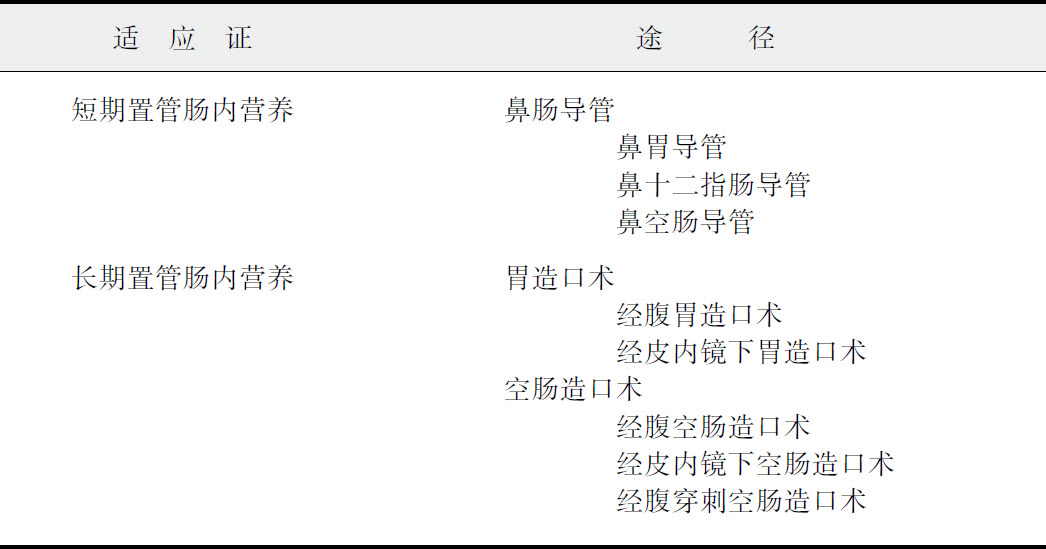
\includegraphics{./images/Image00259.jpg}
\end{table}

\subsubsection{肠内营养制剂应如何选择?}

根据营养素的组成成分,通常将肠内营养制剂分为几种剂型,如整蛋白配方、预消化配方(短肽)以及单体配方(氨基酸为氮源的要素饮食),此外还有接近于正常膳食的匀浆膳和混合奶,重症患者较常选用的为前三者。应依据患者的肠功能状态与所患疾病进行选择,肠功能状态较好的,可选择整蛋模式或肽类(或多聚物配方)肠内营养膳食,否则可选择短肽或结晶氨基酸为氮源的要素饮食。重症胰腺炎及炎性肠道疾病者,可选择氨基酸或短肽为氮源的要素饮食,以减少对胰腺分泌的刺激和肠道消化负担。蛋白质含量较高的膳食发生腹泻的几率增高(图\ref{fig22-1})。

\begin{figure}[!htbp]
 \centering
 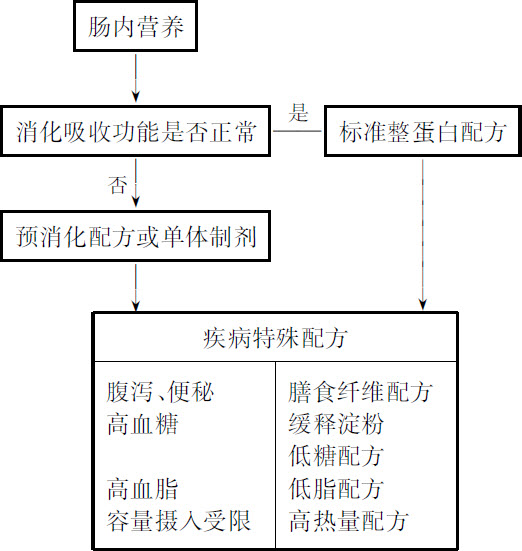
\includegraphics{./images/Image00260.jpg}
 \captionsetup{justification=centering}
 \caption{肠内营养制剂的选择}
 \label{fig22-1}
  \end{figure} 

(1)整蛋白配方 常用酪蛋白及豆蛋白为氮源,多为平衡型肠内营养制剂。营养完全,可口、价廉,蛋白及其他成分在小肠消化吸收,适用于胃肠道消化功能正常者。

(2)预消化配方短肽配方 简单消化即可吸收,极少残渣,粪便形成少,适用于胃肠道有部分消化功能者。

(3)氨基酸单体配方 以氨基酸为蛋白质来源的要素营养,不需胃液、胰液、胆液等参与消化,可直接吸收,不含残渣,粪便形成很少,适用于重症胰腺炎、部分短肠综合征及其他消化功能障碍患者。

上述这些肠内营养的配方又可根据其所含成分进行分类,根据不同疾病状态下的代谢特点及对某些营养素的特殊需要而制成疾病特殊配方的要素饮食,如适应糖代谢异常、呼吸功能障碍、肾衰竭和肿瘤患者的配方,还有适用于重症患者的免疫增强配方的要素饮食。应激较重的重症患者能量消耗增加,可适当增加配方中脂肪的比例,添加支链氨基酸、谷氨酰胺等特需营养成分,以期使肠内营养支持的有效性得到提高。

肠内营养制剂有粉剂与液体制剂两种,配成液体后的热量密度一般为4.2~6.3kJ/ml。

谷氨酰胺是肠黏膜细胞与免疫细胞等的重要能源物质,增加食物中谷氨酰胺的含量,能够促进肠黏膜细胞的防御功能。谷氨酰胺在小肠吸收较好,可促进肠黏膜细胞的生长与防止细菌易位,并通过增加小肠对葡萄糖的吸收和肝细胞对葡萄糖的摄取来调节血糖水平。有关于烧伤患者的临床研究表明,与普通肠内营养制剂相比,谷氨酰胺强化的肠内营养可使感染发生率与病死率明显降低。总的来讲,对于特殊需要,或应用非整蛋白和不含谷氨酰胺的肠内营养制剂的烧伤、创伤等重症患者,补充药理剂量的谷氨酰胺将有助于促进免疫功能及肠黏膜屏障,改善预后,但目前尚没有足够证据表明重症患者肠内营养时需要常规补充谷氨酰胺。

研究表明,膳食中增加ω-3多不饱和脂肪酸(polyunsaturated fatty
acid,富含鱼油),可竞争性地降低前列腺素E\textsubscript{2}
产物的合成,并可减少肿瘤坏死因子和白介素-1、白介素-2、白介素-6的分泌。单核细胞与巨噬细胞是外周细胞中依赖前列腺素E\textsubscript{2}
的主要细胞,极低水平的前列腺素E\textsubscript{2}
有助于淋巴细胞成熟,但高水平的前列腺素E\textsubscript{2}
将抑制细胞的功能。因此,补充ω-3多不饱和脂肪酸能够改善二十烷类物的合成,影响炎症介质、细胞因子的调控,并因此改善免疫代偿和减少机体在严重创伤、感染时的全身炎症反应。

膳食纤维(dietary
fiber)在生理和代谢方面的重要作用愈来愈受到重视,特别是可溶性膳食纤维(如果胶、树胶和植物多糖)在结肠内酵解后可形成短链脂肪酸(short
chain fatty
acid,如丁酸盐、乙酸盐、丙酸盐),进一步影响结肠、小肠的结构与功能;而非可溶性膳食纤维可导致腹胀、粪便干燥和便秘,重症患者应慎用。

\subsubsection{肠内营养引起的并发症有哪些?}

(1)反流、误吸与肺部感染 营养液和消化液的反流、误吸可导致吸入性肺炎。相关因素如下。

肠内营养管移位与折返:一旦发现,即应重新置管及调整位置。

胃排空不良及腹胀:接受食管、胃切除手术使消化道解剖结构发生变化,胃肠运动障碍以及肠内营养应用不当时,可导致消化液、营养液的反流与误吸。这类患者强调营养液肠内输注而不能胃内灌注,营养管尖端位于屈氏韧带以下较为安全。此外,可应用胃动力药物甲氧氯普胺(胃复安)、普瑞博斯(西沙比利)等促进胃的排空及肠蠕动。同时须注意监测患者胃或肠内营养液的潴留量或胃肠减压量与pH。

胃液pH升高:胃液pH升高可导致肠道细菌移位、定植(甚至咽部定植)。有研究认为,24小时持续输注肠内营养液使胃内pH升高,而连续输注16~18小时后,间断8~6小时,则有助于保持胃液的正常酸度,降低肠道菌的移位与口咽部定植,可能有助于降低革兰阴性杆菌的肺部感染发生。

意识障碍:意识障碍患者吞咽、咳嗽反射减退甚至消失,易导致误吸和吸入性肺炎。此时,宜将肠内营养管置于屈氏韧带以下(空肠或幽门以下)十二指肠,且在接受肠内营养治疗时,将头及上半身抬高>30°,需长时间接受肠内营养支持者,可考虑行经皮内镜下胃肠造口术或经皮内镜下空肠造口术。

呼吸道防御能力降低:接受机械通气治疗以及接受咽喉部较大手术的患者,由于气管插管、鼻腔置管或喉返神经损伤,可使吞咽、咳嗽反射减退,呼吸道自我防护能力下降;此外,机械通气的肠内营养患者,十二指肠胃反流较常发生,反流液碱化胃液使pH升高,为了防止此类情况发生,亦应使肠内营养管达到足够深度,以保证营养液从小肠内输注,并注意监测胃内容物酸碱度及残留量。

(2)胃肠不良反应

肠内营养相关腹泻 腹泻是肠内营养较常见的并发症,肠内营养期间发生腹泻的相关因素包括:①配置营养液与开放容器时,造成肠内营养液被污染;②悬挂时间较长或存留有前期未输完的营养液;③营养不良;④低清蛋白血症(清蛋白<25g/L);⑤全身性感染;⑥多器官功能障碍综合征;⑦存在感染灶;⑧发热或低温;⑨应用广谱、强力抗生素。另外,腹泻发生还与营养液输注速度过快、溶液渗透压较高及温度较低等有关。

对于腹泻的防治,应注意以下几方面:①营养液应无菌配制,并置于封闭容器中,每日配制、低温存放,每日更换输注用品;②血浆清蛋白<25g者应先予补充纠正;③适当控制体温,清除体内感染病灶;④输注速度由慢逐渐增加,对于重症患者,最大速度<80ml/小时,一般在60~80ml/小时;⑤若腹泻与抗生素应用有关,则应停用抗生素,并补充双歧杆菌、酵母菌、乳酸杆菌等肠道生态菌;⑥注意输注过程中营养液的温度及浓度,以不同个体能够耐受为标准。

腹胀、便秘和腹痛 重症患者在肠道喂养时易出现不同程度的腹胀,重者使肠内营养无法继续。这类患者在开始肠道喂养时,更应注意减慢输注速度,降低浓度,配合胃肠动力药物及密切监测胃或肠内潴留量,如胃内潴留量>100ml、小肠内潴留量>200ml,应予注意减量或停用。便秘者可增加膳食纤维的补充。

恶心与呕吐 常常是肠内营养液应用不当所致,如灌注速度过快,温度过低,特别是采用间歇性一次性投给喂养方式者。此外,胃肠排空障碍导致的胃、肠内液体潴留,也可导致呕吐。通过调整输注方式、减慢速度等多可得到缓解。

倾倒综合征 放置空肠营养管的重症患者,可出现倾倒综合征,多因高渗溶液快速进入小肠所致。减慢输注速度,适当稀释营养液以降低渗透压,多可使症状缓解。

(3)机械性并发症

肠内营养管堵塞 导管过软(硅胶导管)时易于受折阻塞;配置营养液过稠、未调匀,停止输注后未及时冲洗,添加口服药未充分碾碎或溶解,均可使导管堵塞。配置的营养液室温下放置时间过长可变质形成凝块,冷藏储存者置于过高温度水中加温亦可形成凝块。应用中均要注意予以避免,并在输注前检查营养液的性状。每次/日营养液输注完及注射药物后,均应用>30ml生理盐水或温开水冲洗导管以确保无堵塞。

鼻咽食管和胃黏膜损伤及炎症 留置时间长、管径粗(>12F)、质地硬的导管,可造成鼻腔、咽部、食管黏膜受刺激及黏膜受损,并由此导致炎症,引起鼻炎、咽炎、食管炎及炎性狭窄、胃黏膜炎症、糜烂。鼻黏膜炎症肿胀,可影响鼻窦分泌物引流而发生鼻窦炎,甚至进一步引发颅内感染。对于无症状发热的患者,应注意鼻窦区域的物理检查,必要时可行头颅CT检查。

留置鼻导管者注意鼻咽部分泌物清除,可配合氯霉素与麻黄素滴鼻,以保持鼻窦开口通畅,置管时注意选择导管的型号与材料,减少对局部黏膜的刺激。长期留置营养管的患者可考虑行空肠造瘘。

与经皮内镜下胃或空肠造口术相关并发症 这类并发症包括较严重的有腹壁下脓肿和筋膜坏死,其他还有穿刺造口局部感染、胃液漏出或出血以及气性腹膜炎(可自行缓解)等等。随着内窥镜技术的成熟与经皮内镜下胃肠造口术材料及器械的不断改进,相关并发症已逐渐减少。

(4)代谢性并发症 与肠外营养支持基本相同,包括葡萄糖不耐受、电解质失衡及某些营养素缺乏或过剩等。

\subsubsection{谷胺酰胺如何发挥药理作用?有什么临床意义?}

谷胺酰胺(glutamine,Gln)是体内含量最丰富的非必需氨基酸,大约占骨骼肌内游离氨基酸总量的60%,循环中游离氨基酸总量的20%以上,是蛋白质结构中含量最多的氨基酸。谷氨酰胺是合成蛋白质、核酸和许多其他生物分子的前体,在肝脏、肾脏、小肠和骨骼肌中起着重要的调节作用,是肠黏膜细胞、淋巴细胞、肾小管细胞等许多快速生长细胞或代谢活性细胞的主要能源。

早期研究表明,重症患者应激后血浆谷氨酰胺水平下降为300~400μmol/L(健康人600~700μmol/L),肌肉、游离谷氨酰胺库存的减少是应激性分解代谢的典型特点,谷氨酰胺消耗的比率和病情的严重程度相关。一方面,机体摄入明显减少;另一方面,应激时机体对谷氨酰胺需求明显增加,尽管应激时肌肉组织迅速分解,释放出高于正常3倍的氨基酸,其中1/3为谷氨酰胺。同时肌肉组织中谷氨酰胺合成也随之增加,以供小肠、免疫细胞、脑细胞所需。但是大手术、创伤、烧伤、感染等严重应激状态下,骨骼肌内谷氨酰胺大量释放而被消耗,导致谷氨酰胺缺乏。血浆谷氨酰胺浓度明显下降,肠黏膜萎缩与免疫机能受损。

小肠黏膜是谷氨酰胺代谢的主要部位。谷氨酰胺缺乏,将导致肠上皮萎缩变薄,绒毛变短,黏膜糜烂与溃疡,细胞间连接破坏,使肠通透性增高并导致细菌易位。不论是肠内还是肠外途径补充谷氨酰胺,均可起到促进肠黏膜细胞生长,改善肠黏膜通透性,促进溃疡愈合,维护肠屏障功能,降低腹泻的发生等作用。同时,谷氨酰胺可诱导热休克蛋白表达增加,抑制细胞因子的过多合成,调节全身炎症反应。谷氨酰胺还是免疫细胞的重要能源物质,淋巴细胞、巨噬细胞对谷氨酰胺的利用率较葡萄糖更高,以保证淋巴细胞的增殖和蛋白质合成,修复巨噬细胞的DNA与RNA氧化性损害,提高机体的免疫防御功能,可增强危重症患者对感染的抵抗能力。英国Griffiths
RD的一项单中心、前瞻、双盲研究显示,84例重症医学科重症患者肠外途径补充药理剂量的谷氨酰胺,6个月生存率高于对照组(24/42对比14/42,\emph{P}
=0.049)。法国重症医学科多中心随机对照研究包括了16家医院114例重症患者,与传统全肠外营养相比,谷氨酰胺强化全肠外营养使获得性肺炎与感染发生率明显降低,高血糖发生率低于传统全肠外营养组(\emph{P}
<0.05);需要胰岛素控制血糖的患者数明显减少(14对比22,\emph{P}
<0.05)。但6个月的生存率无明显改善。

对于不能耐受肠内营养的危重症患者,经肠外途径补充谷氨酰胺的效果已从不少的临床事实中得到肯定。谷氨酰胺的药理作用是剂量依赖性的。已制成的谷氨酰胺二肽,如丙氨酰-谷氨酰胺或甘氨酰-谷氨酰胺,解决了谷氨酰胺单体在溶液中不稳定的问题。目前市场上已有商品化的谷氨酰胺二肽单独制剂和含有谷氨酰胺二肽的复方氨基酸溶液,可单独或混合于“全合一”营养液中输注。谷氨酰胺补充应遵循早期、足量(药理剂量)的原则,应用时间一般5~10天。可通过中心静脉或周围静脉输注。谷氨酰胺补充的药理剂量为谷氨酰胺单体每天0.3~0.58g/kg;谷氨酰胺二肽应每天0.5~0.7g/kg,20~40g/天(70kg体重)。

肠内途径补充谷氨酰胺的作用优势为可直接改善肠黏膜上皮的结构与功能。如大面积烧伤患者,肠内营养中添加谷氨酰胺,可获得创面感染率明显降低、住重症医学科与住院时间缩短、住院费用降低的效果。对于某些合并肠屏障功能受损(如炎性肠道疾病等)、谷氨酰胺体内水平较低或丢失过多的接受肠内营养的危重症患者,经肠道补充谷氨酰胺也是需要的。也有研究表明,添加谷氨酰胺的肠内营养,能够明显降低重症急性胰腺炎患者感染性并发症的发生率。感染、多发创伤以及大手术后重症患者,应用谷氨酰胺强化的免疫增强型肠内营养的临床荟萃分析显示
\protect\hyperlink{text00028.htmlux5cux23ch2-27}{\textsuperscript{{[}2{]}}}
,经肠道补充谷氨酰胺有较好的耐受性,能够减轻炎症反应,降低感染性并发症的发生率,降低重症患者的住院时间与医疗费用。

\subsubsection{如何评价鱼油在营养支持中的作用?}

鱼油(ω-3多不饱和脂肪酸)能够通过竞争方式影响传统脂肪乳剂(ω-6
PUFAs)代谢的中间产物(花生四烯酸)的代谢,产生效能不高的“3”系列前列腺素和“5”系列白三烯,使“2”系列的前列腺素如PGE\textsubscript{2}
、PGI\textsubscript{2} 、TXA\textsubscript{2}
等生成减少,“3”系列的前列腺素如PGE\textsubscript{3}
、PGI\textsubscript{3} 、TXA\textsubscript{3}
生成增加;其代谢产物为二十烷五烯酸(EPA)和二十二烷六烯酸(DHA),具有降低炎症反应与较少免疫抑制的生理效应,从而有助于下调过度的炎症反应,促进巨噬细胞的吞噬功能,改善免疫机能。

ω-3多不饱和脂肪酸还可影响细胞膜的完整性、稳定性和流动性,影响细胞运动、受体形成、受体与配体的结合等,从而减少细胞因子的产生和释放,有助于下调炎症反应,促进巨噬细胞的吞噬功能,改善免疫功能,有助于维持危重疾病状态下血流动力学稳定。对代谢方面影响的为ω-3多不饱和脂肪酸对脂肪、糖及蛋白质代谢亦具有一定的调理作用,通过增加血脂的分解与清除以及影响脂蛋白的合成,降低低密度脂蛋白、极低密度脂蛋白的合成及其受体活性,增加高密度脂蛋白受体活性,影响机体对脂肪的利用。通过增加外周组织对葡萄糖的摄取及其氧化,有助于改善应激后糖的代谢。并可能通过对炎症介质分泌的影响,降低肿瘤坏死因子(TNF)α、白细胞介素(IL)-1、白细胞介素(IL)-2、白细胞介素(IL)-6的分泌,从而降低创伤、感染后机体的炎症反应及机体的能量代谢,降低体内蛋白质消耗、促进蛋白质合成,改善氮平衡。

已有研究表明,重症急性胰腺炎病人在疾病早期应用添加鱼油的肠外营养支持可减低机体过度炎症反应
\protect\hyperlink{text00028.htmlux5cux23ch4-27}{\textsuperscript{{[}4{]}}}
,改善肺的氧合功能。有关急性肺损伤和ARDS的研究显示,ω-3多不饱和脂肪酸可使肺动脉压下降、肺血管通透性改善,由此改善肺功能、缩短机械通气时间与住重症医学科时间。接受全肠外营养治疗的661例腹部大手术
\protect\hyperlink{text00028.htmlux5cux23ch5-27}{\textsuperscript{{[}5{]}}}
、腹腔感染以及包括颅脑外伤在内的多发创伤等危重症患者
\protect\hyperlink{text00028.htmlux5cux23ch6-27}{\textsuperscript{{[}6{]}}}
,添加药理剂量的鱼油脂肪乳剂3天以上,患者生存率得到明显改善,抗生素使用与感染的发生率降低,住院时间缩短。鱼油改善预后的效果亦呈现剂量依赖的特点,有效药理剂量为每天0.1~0.2g/kg。最近的研究显示,补充ω-3多不饱和脂肪酸能够改善ARDS患者的肺部炎症反应,并能够明显改善氧合。

肠外与肠内途径补充ω-3多不饱和脂肪酸均可调控重症患者的免疫炎症反应
\protect\hyperlink{text00028.htmlux5cux23ch7-27}{\textsuperscript{{[}7{]}}}
,有可能改善重症患者预后
\protect\hyperlink{text00028.htmlux5cux23ch8-27}{\textsuperscript{{[}8{]}}}
。ω-3多不饱和脂肪酸的临床效应与疾病严重程度有关,在炎症反应不甚严重和不合并器官功能障碍的患者,补充ω-3多不饱和脂肪酸似乎并无优势。目前尚无ω-3多不饱和脂肪酸能够改善全身性感染和感染性休克等危重症患者预后的有力证据。

\subsubsection{合并急性呼吸衰竭的重症患者营养支持有何特点?}

急性呼吸窘迫综合征(ARDS)是由肺部原发疾病或肺外疾病导致的肺部炎症反应,进而导致的肺泡渗液增加、血氧下降、呼吸窘迫的一种综合征。不同于其他类型的急性呼吸衰竭(如急性肺栓塞、支气管哮喘急性发作),ARDS存在着明显的全身炎症反应,并伴随着体内各种应急激素及多种细胞因子和炎症介质的释放。

(1)ARDS的代谢特点 由于创伤、感染等原发疾病或损害(如严重创伤、感染,重症胰腺炎等),导致ARDS患者出现严重的高分解代谢,能量消耗增加,加之多数患者需要机械通气治疗,其静息能量消耗可达预计值的1.5~2倍,患者迅速出现营养不良。脂肪动员,瘦体组织分解,各种结构与功能蛋白被迅速消耗,血清白蛋白下降、谷氨酰胺明显减少,血中氨基酸比例失调。

(2)ARDS患者的营养支持原则 尽早实施营养支持可缩短接受机械通气患者的上机时间,改善营养与免疫状态,缩短住重症医学科时间,降低医疗费用。如患者肠道功能允许,应尽快建立胃肠通道,早期给予肠内营养,并采取充分的措施避免反流和误吸。

应注意的是:①呼吸衰竭患者应避免过度喂养,特别是碳水化合物补充过多将增加二氧化碳的产生、增加呼吸商、加重患者的呼吸负荷。可适当增加非蛋白质热量中脂肪的比例。②多项1级临床研究表明,ARDS患者接受肠内营养并联合二十烷五烯酸(EPA)以及抗氧化物质的肠内营养支持,可以提高体内的抗氧化水平,防止脂质过氧化损害,减少支气管肺泡灌洗液中中性粒细胞数量,降低肺血管阻力与肺泡通透性,改善肺功能,改善气体交换,从而缩短上机时间和重症医学科停留时间,减少进一步的器官功能损伤。来自欧洲的一项大样本、多中心、随机研究表明
\protect\hyperlink{text00028.htmlux5cux23ch6-27}{\textsuperscript{{[}6{]}}}
:165例感染与感染性休克接受机械通气的重症患者,应用添加鱼油、亚麻酸及抗氧化维生素的肠内营养支持,明显改善了28天存活率,并缩短了机械通气时间与住重症医学科天数
\protect\hyperlink{text00028.htmlux5cux23ch9-27}{\textsuperscript{{[}9{]}}}
。因此,合并ARDS患者营养支持的原则应掌握:①尽早给予营养支持,并首选肠内营养;②适当降低非蛋白热量中碳水化合物的比例,降低呼吸商;③添加含鱼油与抗氧化剂的营养配方。这可能成为合并呼吸衰竭的重症患者更理想的营养支持方式。

\subsubsection{重症患者实行强化胰岛素治疗有哪些临床意义?如何实施?}

应激性高血糖是重症医学科中普遍存在的一种临床现象,即使是以往无糖尿病史的重症患者,并且血糖升高已成为一独立因素直接影响重症患者的预后。多项前瞻性与回顾性临床研究表明,严格血糖控制可改善各类重症医学科重症患者的预后。特别是外科重症患者,严格血糖控制可使因严重感染导致多器官功能衰竭患者的病死率明显降低,使其他并发症的发生率亦有明显下降,如严重感染、需要血液净化治疗的急性肾衰竭患者的发生率,以及多神经病变等。缩短机械通气时间与住院时间,从而降低总住院费用。进一步分析显示,对于住重症医学科超过5天的重症患者,严格控制血糖水平(≤6.1mmol/L),对病死率的改善作用更为明显。对于非手术的内科重症患者的研究显示,严格控制血糖,虽然总的病死率尚未获得有统计学意义的改善,但在降低医院内获得性肾损害的发生率、缩短机械通气时间和重症医学科住院天数等方面,仍可获得有显著意义的改善。因此,正确处理各类重症患者的应激性高血糖,对于提高其综合治疗效果,改善生存率具有重要的意义。任何形式的营养支持均应包括强化胰岛素治疗,严格将血糖控制在理想范围
\protect\hyperlink{text00028.htmlux5cux23ch10-27}{\textsuperscript{{[}10{]}}}
\textsuperscript{,}
\protect\hyperlink{text00028.htmlux5cux23ch11-27}{\textsuperscript{{[}11{]}}}
。但是近来多项研究发现严格控制血糖可能会增加严重低血糖风险(40mg/dl),因此目前重症病人的血糖控制推荐意见为:①重病患者的血糖控制应使用胰岛素,不建议使用其他药物控制血糖;②重病患者血糖控制应尽量维持平稳,避免大幅度波动;③目标血糖标准在6.1~8.3mmol/L,可获得明确的改善重症患者预后的效果,同时可减少低血糖的不良事件的发生。

\subsubsection{重症患者实行强化胰岛素治疗中需注意哪些问题?}

在强化胰岛素治疗中应当注意:

(1)由于应激性高血糖主要表现为以外周胰岛素抵抗为特征的血糖升高,并且血糖增高的程度与应激、疾病严重程度成正比。由于重症患者病情的多变以及治疗措施的多变性,增大了血糖控制难度。因此,在实施强化胰岛素治疗期间,应当密切监测血糖,及时调整胰岛素用量,防止低血糖发生。

(2)重症患者的营养支持中,非蛋白质热量中的葡萄糖含量与输注速度直接影响着患者的血糖水平。一般情况下,葡萄糖的输入量应当控制在≤200g/天。营养液以外的治疗尽量应用无糖液体(如抗生素溶液),以免增加血糖的波动。

(3)营养液的输入应当注意持续、匀速,葡萄糖与胰岛素按比例补充。

(4)合并感染与应用影响糖代谢药物时(如糖皮质激素、生长激素、生长抑素等),注意血糖的检测及增加胰岛素用量。

(5)严密的血糖监测是实现安全有效血糖控制的保证。

总之,任何形式的营养支持,应配合强化胰岛素治疗,严格控制血糖水平,并应注意避免低血糖发生。

\begin{center}\rule{0.5\linewidth}{\linethickness}\end{center}

参考文献

\protect\hyperlink{text00028.htmlux5cux23ch1-27-back}{{[}1{]}} .Bongers
T,Griffiths RD.Are there any real differences between enteral feed
formulations used in the critically ill?Curr Opin Crit
Care,2006,12:131-135.

\protect\hyperlink{text00028.htmlux5cux23ch2-27-back}{{[}2{]}} .Miller
KR,Kiraly LN,Lowen CC,et al.“CAN WEFEED?”A Mnemonic to Merge
Nutrition and Intensive Care Assessment of the Critically Ill Patient.J
PEN 2011,35(5):643-659.

\protect\hyperlink{text00028.htmlux5cux23ch3-27-back}{{[}3{]}} .Casaer
MP,Mesotten D,Hermans G,et al.Early versus late parenteral nutrition
in critically ill adults.N Engl J Med.2011,365(6):506-517.

\protect\hyperlink{text00028.htmlux5cux23ch4-27-back}{{[}4{]}}
.{Xinying Wang} ,Weiqin Li,Feng Zhang,Liya Pan,Ning Li,Jieshou
Li.Fish oil-supplemented parenteral nutrition in severe acute
pancreatitis patients and effects on immune function and infectious
morbidity:a randomized controlled
trial.Inflammation,2009,32(5):304-309.

\protect\hyperlink{text00028.htmlux5cux23ch5-27-back}{{[}5{]}}
.Garcia-de-Lorenzo A,Zarazaga A,Garcia-Luna PP,et al.Clinical
evidence for enteral nutritional support with glutamine:a systematic
review.Nutrition,2003,19:805-811.

\protect\hyperlink{text00028.htmlux5cux23ch6-27-back}{{[}6{]}} .Villet
S,Chiolero RL,Bollmann MD,et al.Nagative impact of hypocaloric
feeding and energy balance on clinical outcome in ICU patients.Clin
Nutrition,2005,24:502-509.

\protect\hyperlink{text00028.htmlux5cux23ch7-27-back}{{[}7{]}}
.{Xinying Wang} ,Weiqin Li,Ning Li,Jieshou Li.ω-3 fatty acids
supplemented parenteral nutrition decreases hyperinflammatory response
and attenuates systemic disease sequelae in severe acute pancreatitis
--- a randomized and controlled study.Journal of Parenteral and Enteral
Nutrition,2008,32(3):236-241.

\protect\hyperlink{text00028.htmlux5cux23ch8-27-back}{{[}8{]}} .Heller
AR,Rossler S,Litz RJ,et al.T.Omega-3 fatty acids improve the
diagnosis-related clinical outcome.Crit Care Med,2006,34:972-979.

\protect\hyperlink{text00028.htmlux5cux23ch9-27-back}{{[}9{]}}
.Pontes-Arruda A,Aragao AM,Albuquerque JD.Effects of enteral feeding
with eicosapentaenoic acid,gamma-linolenic acid,and antioxidants in
mechanically ventilated patients with severe sepsis and septic
shock.Crit Care Med.2006,34:2325-2333.

\protect\hyperlink{text00028.htmlux5cux23ch10-27-back}{{[}10{]}} .Van
den Berghe,Wouters PJ,Bouillon R,et al.Outcome benefit of intensive
insulin therapy in the critically ill.Crit Care
Med,2003,31:359-366.

\protect\hyperlink{text00028.htmlux5cux23ch11-27-back}{{[}11{]}} .Van
den Berghe,Wilmer A,Hermans G,et al.Intensive Insulin Therapy in the
Medical ICU.N Engl J Med,2006,354:449-461.

\protect\hypertarget{text00029.html}{}{}

